\rule{0.5\textwidth}{0.5pt}\\

	{\large \textbf{EXPERIMENT NewFluxAutoencoder10000-1}}\\
	
	{\normalsize HYPERPARAMETERS:}
	\begin{lstlisting}
	*ARCHITECTURE HYPERPARAMETERS:
		-Autoencoder
		-Input shape: (56, 24, 1)
		-Convolutional Layers: [512, 128, 64, 8]
			(Inverse in the decoder)
		-Convolutonal Kernels: [(3, 3), (3, 3), (3, 3), (3, 3)] 
			(Inverse in the decoder)
		-Convolutional Activation: relu
		-Output Layer Activation: linear
		-Padding: same
		-Use Batch Normalization: True
	
	*COMPILATION HYPERPARAMETERS:
		-Optimizer: ADAM lr=0.001, beta_1=0.9, beta_2=0.999
		-Loss Function: MSE
		-Metric: MSE
	
	*TRAINING HYPERPARAMETERS:
		-Epochs: 75
		-Batch size: 32
		-Callbacks:
			-ReduceLROnPlateau: MSE 8 x0.1
			-Early Stop: MSE 15
	\end{lstlisting}
	
	{\normalsize VISUALIZATION:}
	\begin{lstlisting}
	*RESULTS:
        -Train MSE: 0.0018673702143132687
        -Validation MSE: 0.005482238717377186
	\end{lstlisting}
	
	\begin{figure*}[ht!]
		\subfloat[Training Evolution]{%
		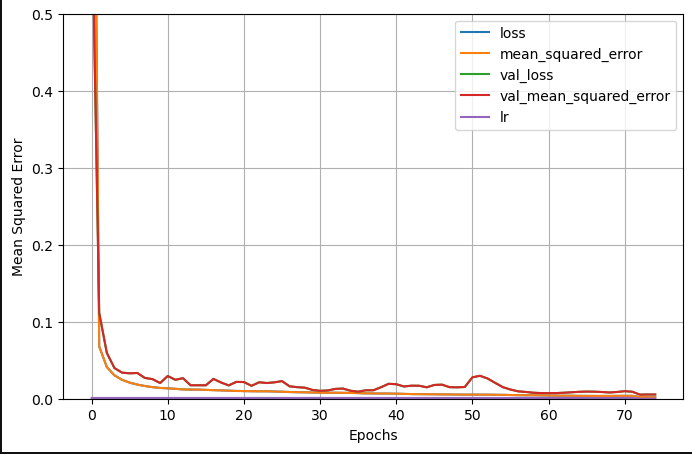
\includegraphics[ width=0.31\textwidth]{ap-NewFluxAutoencoder10000-1-evolution.png}}
		\hspace{\fill}
		\subfloat[Validation example]{%
		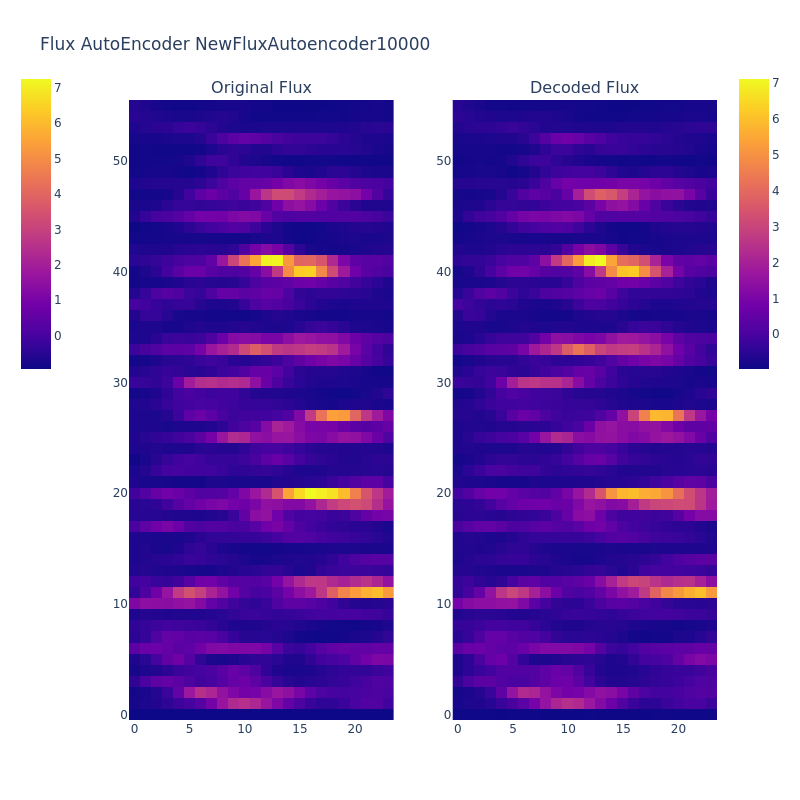
\includegraphics[ width=0.31\textwidth]{ap-NewFluxAutoencoder10000-1-val.png}}
		\hspace{\fill}	
		\subfloat[Train example]{%
		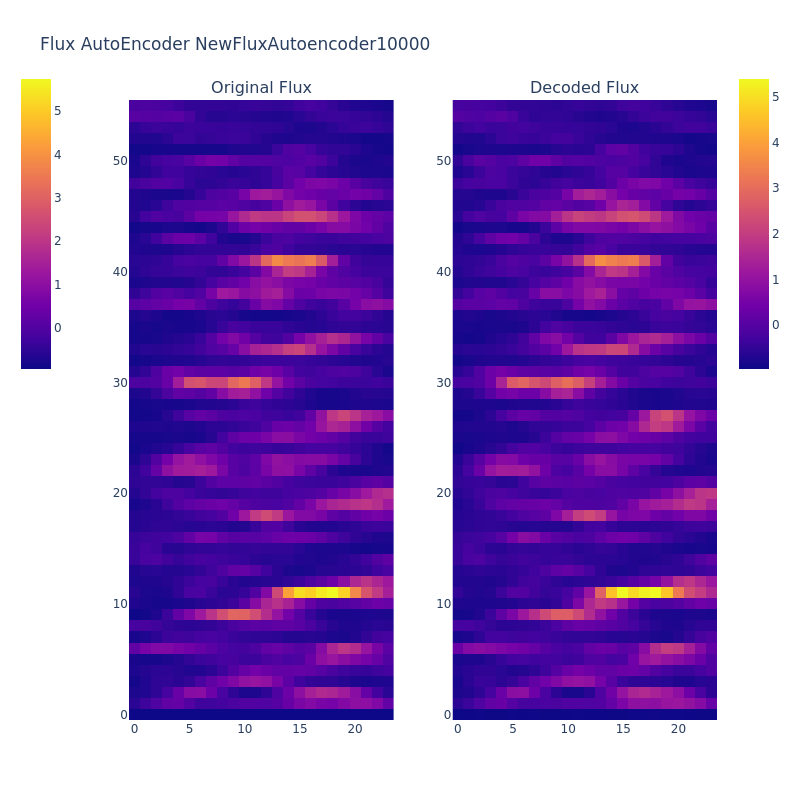
\includegraphics[ width=0.31\textwidth]{ap-NewFluxAutoencoder10000-1-train.png}}\\
		\caption{Results of training the model NewFluxAutoencoder10000-1}
	\end{figure*}
	
\FloatBarrier	
\rule{0.5\textwidth}{0.5pt}\\